\begin{frame}[fragile]{Überblick}
\begin{itemize}
\item Historie
\item Konzepte
\item Demo
\end{itemize}
\end{frame}


\begin{frame}[fragile]{Historie}
\begin{itemize}
\item 2008: Projekt mit monatlicher Metrik-Ermittlung
\onslide+<2->
\item Wunsch nach schnellerem Feedback-Zyklus 
\begin{itemize}
\item $\Rightarrow$ Einsicht
\end{itemize}
\onslide+<3->
\item Wunsch nach Hilfestellung bei der Problembehebung 
\begin{itemize}
\item $\Rightarrow$ Handeln
\end{itemize}
\end{itemize}
\end{frame}

\begin{frame}[fragile]{Unsere Grundannahmen}

\begin{itemize}
\item Softwareentwicklung ist holistisch
\begin{itemize}
\item Betrachten von Teilen erlaubt Rückschlüsse auf das Ganze
\end{itemize}
\end{itemize}

\begin{itemize}
\item Qualität von Code, Design und Architektur hängen zusammen
\end{itemize}
\end{frame}

\begin{frame}[fragile]{Unsere Ziele}

\begin{itemize}
\item Wir wollen handeln statt nur zu messen
\item Handeln muss so einfach wie möglich sein
\end{itemize}

\end{frame}

\begin{frame}[fragile]{Unsere Designentscheidungen}
\begin{itemize}
\item Nur wenige Metriken mit großer Nähe zum Code
\item Metriken, die uns nahelegen, wie wir handeln können
\item Keine speziellen OO-Metriken
\begin{itemize}
\item Geeignet für alle Arten von Java-Code
\end{itemize}
\item In IDE integriert
\item Hotspots zeigen die kritischen Stellen
\end{itemize}

\end{frame}


\begin{frame}[fragile]{Demo}
\begin{center}
{\Huge Demo}
\end{center}
\end{frame}

%%%%%%%%%%%%%%%%%%%%%%%%%%%%%%%%%%%%%%%%%%%%%%%%%%
{
%\usebackgroundtemplate{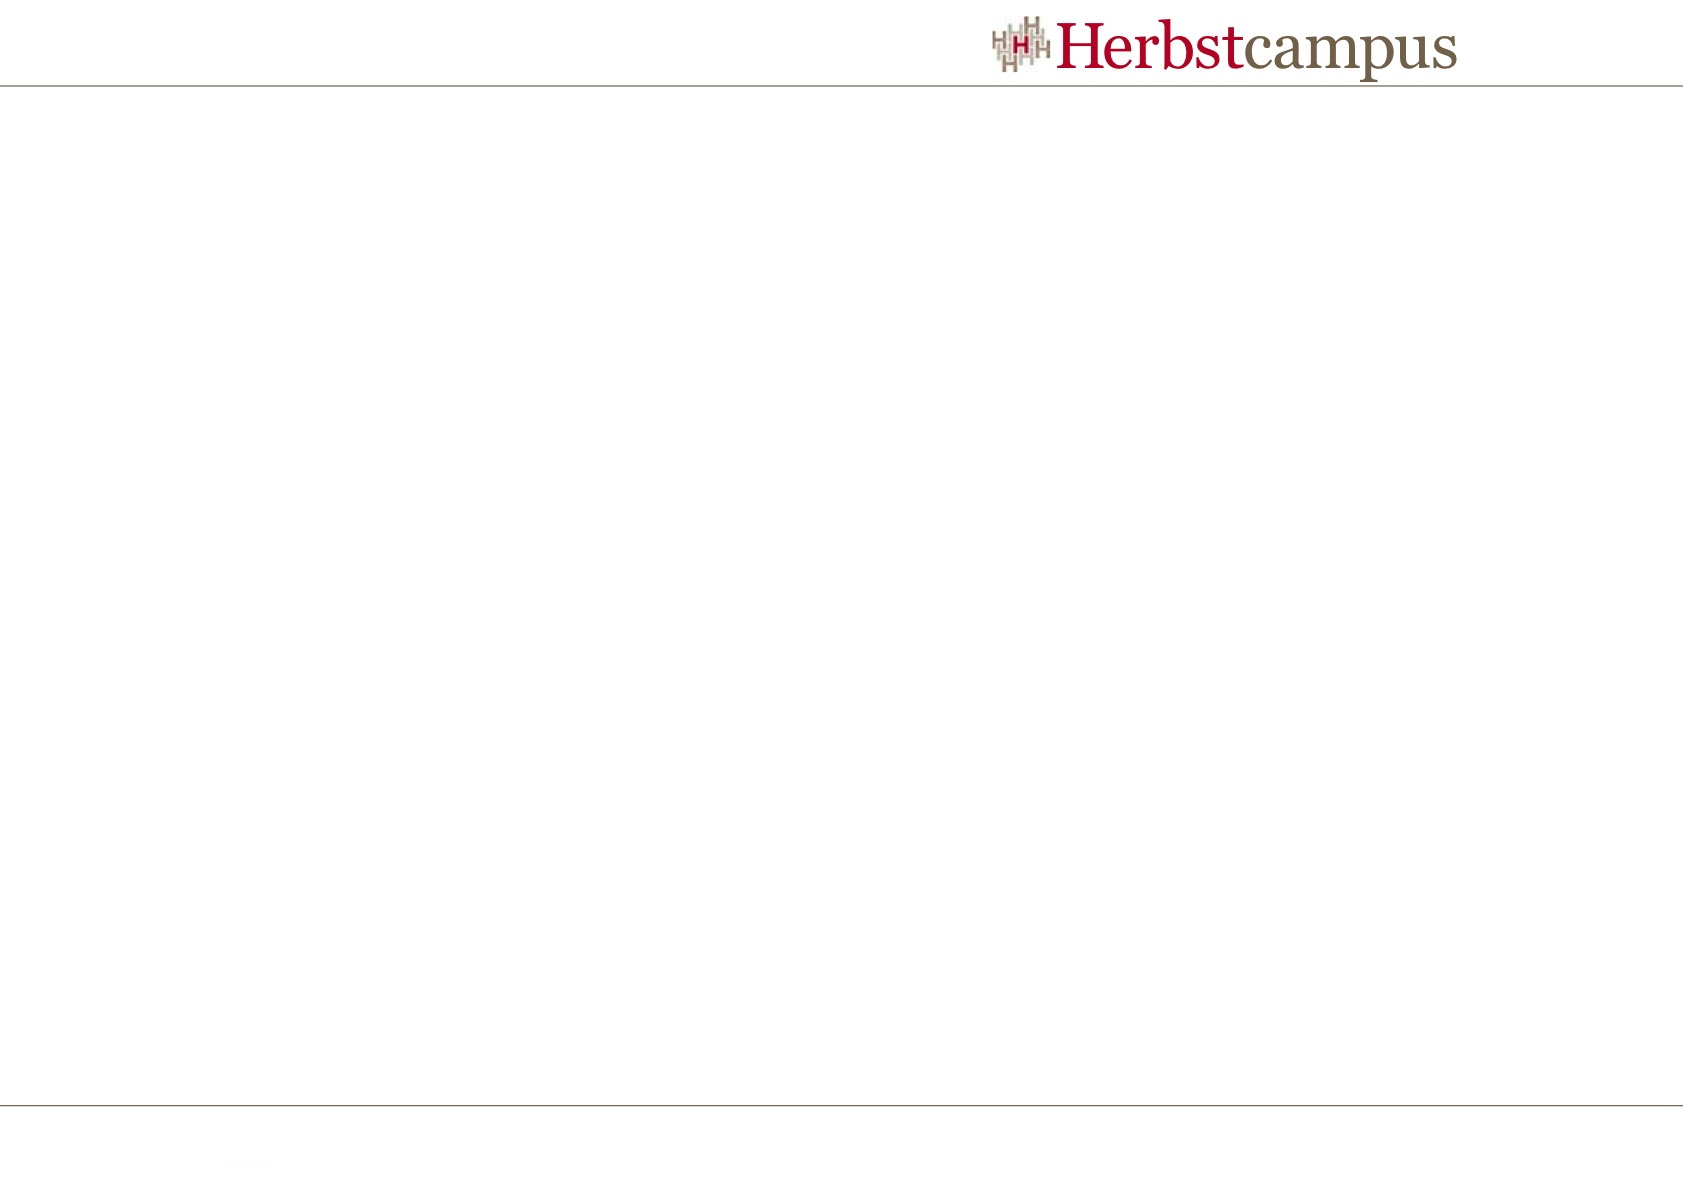
\includegraphics[width=\paperwidth,height=\paperheight]{background-slide.png}}
\begin{frame}{Vielen Dank!}

        Folien auf GitHub:
        \begin{center}
                \url{https://github.com/projectusus/org.projectusus.documentation/Vortrag Herbstcampus 2013}
        \end{center}

        \begin{block}{Nicole Rauch}
        \begin{description}[Twitterxx]
                \item[E-Mail]  \href{mailto:nicole.rauch@msg-gillardon.de}{\texttt{nicole.rauch@msg-gillardon.de}}
                \item[Twitter] \href{http://twitter.com/NicoleRauch}{\texttt{@NicoleRauch}}
        \end{description}
        \end{block}
\end{frame}
}
